\documentclass[fleqn,usenatbib]{acmart}
\usepackage{newtxtext,newtxmath}
\usepackage{pict2e}
\usepackage[greek,english]{babel}
\usepackage[T1]{fontenc}
\usepackage{tikz}
\usepackage{pgfplots}
\usetikzlibrary{decorations.pathreplacing,calligraphy,patterns}
% \usepackage{../../Papers/JML}
%%%%% copying the contents of the Jack Markup Library here for transport
	\usepackage{environ}
	\renewcommand{\d}{\mathrm d}
	\newcommand{\eref}[1]{Eq. \eqref{#1}}
	\renewcommand{\div}[2]{\frac{\d #1}{\d #2} }
	\newcommand{\pdiv}[2]{\frac{\partial #1}{\partial #2}}
	\def\LLR
	{
		~~\Longleftrightarrow~~
	}
	\def\LR
	{
		~~~\Longrightarrow~~~
	}

	\NewEnviron{spalign}
	{
		\begin{align}
			\begin{split}
				\BODY
			\end{split}
		\end{align}
	}


%%%% continuing on from here
\bibliographystyle{unsrtnat}
\citestyle{acmnumeric}
\title[GeneCHORD]{\codename{}: A Pipeline for Genomic Rearrangement Analysis}
\author{Jack Fraser-Govil}
\author{Ronnie Crawford}
\affiliation{
   \institution{Wellcome Sanger Institute}
   \city{Hinxton}
   \country{United Kingdom}
%    \postcode{CB10 1RQ}
}
\author{Max Stammnitz}
\author{Elizabeth Murchison}
\affiliation{
   \institution{University of Cambridge}
   \city{Cambridge}
   \country{United Kingdom}
%    \postcode{CB10 1RQ}
}
\author{Zemin Ning}
\affiliation{
   \institution{Wellcome Sanger Institute}
   \city{Hinxton}
   \country{United Kingdom}
   \postcode{CB10 1RQ}
}
\def\commentVisible{1}

\def\codename{\textit{GenCHORD}}


\begin{document}

	% \label{firstpage}
	
	\begin{abstract}
		We present \codename{}, a specialised step-detection algorithm suitable for detecting large-scale copy number variations from the coverage data of a sequenced, aligned genome. This algorithm is specifically tuned for detecting Structural Variations which arise during chromothripsis-induced cancer, and so permits a high degree of data reduction, whilst preserving pertinent features for cancer classification. We describe the underlying statistical and algorithmic model, demonstrate the ability of the to preserve, compress and encode information such that a simple Machine Learning model can classify and identify subtypes of Devil Facial Tumour Disease, a cancer affecting \textit{Sarcophilus harrisii}, the Tasmanian Devil, and discuss how this tool may be used in future.   
	\end{abstract}
	\maketitle

	\newcommand\new[1]
	{
		{\color{red} #1}
	}

	\section{Introduction}
	
		{The term} Genomic Rearrangements refer to large-scale Structural Variations (SVs) amongst individual genomes; including large-scale deletion, insertion, duplication and translocation of megabase-length sequences of DNA,  and often lead to genetic disorders (when present in the germ cells), or cancer (when arising from somatic mutations). When a Genomically Rearranged sample is sequenced and aligned against a reference the true sequences novel adjacencies can be obscured, especially when the size of the rearranged regions are significantly larger than the read length. This is because the majority of  reads will still align to the reference despite the fact that their spatial location within the genome has been altered: only those reads which bridge the unusual adjacencies contain the information that a rearrangement has occurred.

		Reconstructing these rearrangements requires complex analysis, such as a haplotype phased-assembly , which is not only computationally costly, but requires the DNA be sequenced to a very high coverage, as well techniques such as Hi-C\cite{Ijaz2024}. We should like to be able to identify, analyse and classify the presence of genomic rearrangements in a simpler fashion.  

		To do this, we leverage the knowledge that chromothripsis-induced rearrangements are often associated with highly variable copy-number variations\cite{Ijaz2024,Chromo2011}. Where portions of the genome have been duplicated or deleted (generically termed 'gains' and 'losses'), the erroneous alignment leads to variations in the base-coverage reported by the alignment tool, as demonstrated in Figure \ref{Fig:Diagram}. {The locations of regions which have undergone gains and losses corresponds strongly to the edges of the regions which have been rearranged.}

		Many tools to analyse the copy-number variations exist, however in this work we develop \textbf{Gen}ome \textbf{C}overage \textbf{H}armonic \textbf{O}ptimiser, \textbf{R}educer and \textbf{D}e-noiser (\codename{}), a novel tool tailored for this problem which leverages the power of a Bayesian hypothesis testing to infer a statistically robust denoised copy-number analysis, which is suitable for encoding into a Neural Network, and hence permit accurate detection, analysis, and classification of the genomic rearrangement.

		\begin{figure}
			\begin{center}
				\resizebox{!}{5cm}{ 
				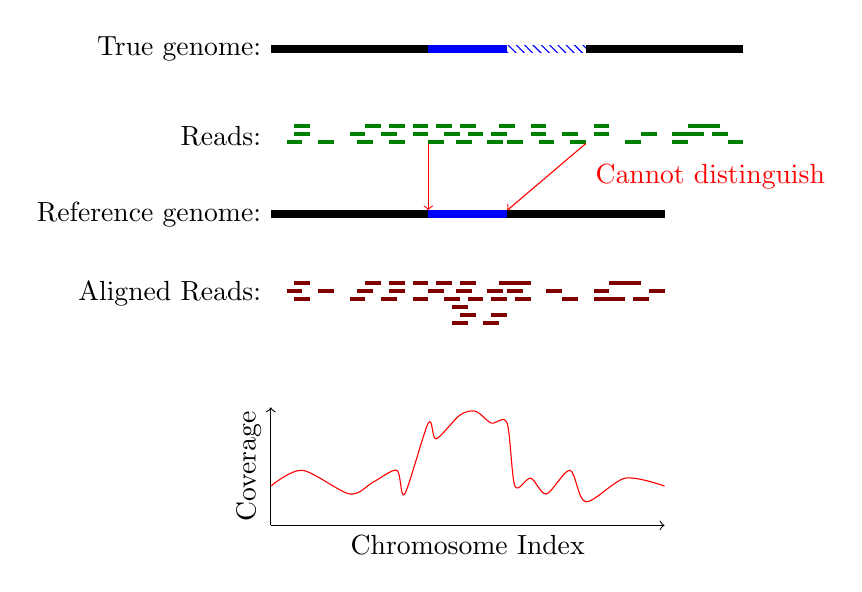
\begin{tikzpicture}
					\node[anchor=east] at (0,0.05) {True genome:};
					\fill (0,0) rectangle (2,0.1);
					\fill[blue] (2,0) rectangle (3,0.1);
					\fill[blue,pattern=north west lines, pattern color=blue] (3,0) rectangle (4,0.1);
					\fill (4,0) rectangle (6,0.1);

					\def\readheight{-1}
					\node[anchor=east] at (0,{\readheight-0.05}) {Reads:};

					\foreach[count=\i] \x in {0.3,1,1.4,1.8,2.2,2.5,2.8,3.3,3.7,4.1,4.7,5.1,5.3,5.6}
					{
						\fill[green!50!black] (\x,\readheight) rectangle ({\x+0.2},{\readheight -0.05});
					}
					\foreach[count=\i] \x in {0.2,0.6,1.1,1.5,2,2.35,2.75,3,3.4,3.8,4.5,5.1,5.8}
					{
						\fill[green!50!black] (\x,{\readheight-0.1}) rectangle ({\x+0.2},{\readheight -0.15});
					}
					\foreach[count=\i] \x in {0.3,1.2,1.5,1.8,2.1,2.4,2.9,3.3,4.1,5.3,5.5}
					{
						\fill[green!50!black] (\x,{\readheight+0.1}) rectangle ({\x+0.2},{\readheight +0.05});
					}
					\def\refheight{-2}
					\draw[->,red] (2,\readheight-0.15)--(2,\refheight);
					\draw[->,red] (4,\readheight-0.15)--(3,\refheight);
					\node[anchor=west,red] at (4,{(\refheight+\readheight-0.15)/2}) {Cannot distinguish};
					\node[anchor=east] at (0,{\refheight -0.05}) {Reference genome:};
					\fill (0,\refheight) rectangle (2,{\refheight -0.1});
					\fill[blue] (2,\refheight) rectangle (3,{\refheight -0.1});
					\fill (3,\refheight) rectangle (5,{\refheight -0.1});

					\def\areadheight{-3}
					\node[anchor=east] at (0,{\areadheight-0.05}) {Aligned Reads:};

					\foreach[count=\i] \x in {0.3,1,1.4,1.8,2.2,2.5,2.8,3.3,3.7,4.1,4.7,5.1,5.3,5.6}
					{
						\def\xoffset{0}
						\def\yoffset{0}
						\newdimen\pos
						\pos = \x cm
						\ifdim \pos > 3cm
							\def\xoffset{1}
							\ifdim \pos < 4cm
								\def\yoffset{0.3}
							\fi
						\fi
						\fill[red!50!black] ({\x-\xoffset},{\areadheight -\yoffset-0.1}) rectangle ({\x-\xoffset+0.2},{\areadheight -\yoffset-0.15});
					}
					\foreach[count=\i] \x in {0.2,0.6,1.1,1.5,2,2.35,2.75,3,3.4,3.8,4.5,5.1,5.8}
					{
						\def\xoffset{0}
						\def\yoffset{0}
						\newdimen\pos
						\pos = \x cm
						\ifdim \pos > 3cm
							\def\xoffset{1}
							\ifdim \pos < 4cm
								\def\yoffset{0.3}
							\fi
						\fi
						\fill[red!50!black] ({\x-\xoffset},{\areadheight -\yoffset}) rectangle ({\x-\xoffset+0.2},{\areadheight -\yoffset-0.05});
					}
					\foreach[count=\i] \x in {0.3,1.2,1.5,1.8,2.1,2.4,2.9,3.3,4.1,5.3,5.5}
					{
						\def\xoffset{0}
						\def\yoffset{0}
						\newdimen\pos
						\pos = \x cm
						\ifdim \pos > 3cm
							\def\xoffset{1}
							\ifdim \pos < 4cm
								\def\yoffset{0.3}
							\fi
						\fi
						\fill[red!50!black] ({\x-\xoffset},{\areadheight -\yoffset+0.1}) rectangle ({\x-\xoffset+0.2},{\areadheight -\yoffset+0.05});
					}


					\def\plotheight{-6}
					\draw[->](0,\plotheight)--(5,\plotheight);
					\draw[->](0,\plotheight)--++(0,1.5);
					\draw [red] plot [smooth] coordinates {(0,{\plotheight+0.5}) (0.4,{\plotheight+0.7}) (1,{\plotheight+0.4}) (1.3,{\plotheight+0.55}) (1.6,{\plotheight+0.7}) (1.7,{\plotheight+0.4})
						(2,{\plotheight+1.3})  (2.1,{\plotheight+1.1})  (2.4,{\plotheight+1.4})  (2.6,{\plotheight+1.45}) (2.8,{\plotheight+1.3})	(3,{\plotheight+1.3})  
						(3.1,{\plotheight+0.5}) (3.3,{\plotheight+0.6}) (3.5,{\plotheight+0.4}) (3.8,{\plotheight+0.7}) (4,{\plotheight+0.3}) (4.5,{\plotheight+0.6})  (5,{\plotheight+0.5})    
						};

					\node[anchor=north] at (2.5,\plotheight) {Chromosome Index};
					\node[anchor=south,rotate=90] at (0,{\plotheight+0.75}) {Coverage};
				\end{tikzpicture}
				}
			\end{center}\caption{A depiction of duplication leading to a higher coverage. The blue hatched region is duplicated with respect to the reference, but since the reads are much shorter than the duplicated region, they manifest as a higher coverage rate.}\label{Fig:Diagram}
		\end{figure}

	\section{Statistical Theory \& Algorithm}

		\subsection*{The Data}

			Throughout this work we shall assume that our data is the coverage (per-base sequencing depth) extracted from an aligned BAM file\footnote{such as with the samtools \textit{depth} command}. Our data therefore takes the form of an ordered sequence of integers, $S = \{k_1,k_2,k_3,...\}$, where $k_i$ is a nonnegative integer corresponding to the coverage reported by the $i^\text{th}$ base in the sequence.
			
			We shall have $C$ such sequences, corresponding to the $C$ {distinct} chromosomes present in the sample. Each sequence is of length $N_c$ (the length of the $c^\text{th}$ chromosome). We shall assume that, aside from a prior that the global parameters should be similar\footnote{But not identical, since the coverage depth can vary per-chromosome in even a healthy sample}, these sequences are to be analysed independently.

			The values of $k$ are distributed around a central value by a degree of noise arising from biological variation and experimental error in the pipeline. Where this central value undergoes a drastic, discontinuous change is indicative of the beginning of a gain or a loss, and hence (in the context of chromothripsis) a region which has undergone rearrangement.

		\subsection{Smoothing \& Binning}

			{The most obvious solution to denoise the Coverage Data is to simply pass a smoothing kernel over the data, potentially in combination with a binning algorithm, and use that to infer the underlying mean function that the data is oscillating around. Smoothing in this fashion serves as a generic way to extract a smooth curve from the extremely noisy data present, however it fails us on a number of grounds. Most importantly, this method can act to bias and manipulate the data in unforeseen and undesirable ways. Anecdotally, we found many occasions where the severity of an inferred deletion or duplication could be manipulated by altering the analysis lengthscale. }
			
	


		\subsection{Harmonic Fitting}

			% The primary problem with the na\"ive smoothing approach was that it (by definition) \textit{smoothed out} the data, in order that we might more easily spot \textit{discontinuities} in the data. These two points -- smoothing and discontinuities -- stand in direct opposition to each other, and so the method is inherently flawed.

			We should therefore attempt to identify the coverage-discontinuities directly from the dataset. This, in essence is a form of \textit{step detection}, a well known problem in signal processing. However, whilst there exist several out-of-the-box algorithms which might provide us with robust detections, we note that knowledge about the form of the data can be leveraged to provide a significantly more powerful and biologically meaningful inference. 
			
			\subsubsection{Model Assumptions}
			
				We use the following knowledge and assertions as the underpinnings of our model.

				Firstly, as argued in Appendix \ref{A:Theory}, we assume that the coverage, $k$, is distributed according to a (slightly modified) Negative Binomial probability mass function, which is characterised by the mean $\mu$ and variation $\sigma^2_\text{model} = \mu + \sigma^2$, where $\sigma^2 > 0$ is the variation associated with the biological variability.
	
				% That is, $\mathcal{P}$ is the Negative Binomial distribution with mean equal to the mean of the error function, $\mu_\text{model} = \mu$, and the variance equal to $\sigma^2_\text{model} = \mu + \sigma^2$. We will use $\sigma$, rather than $\sigma_\text{model}$ throughout as it is independent of the mean and is only constrained to be positive, rather than $\sigma_\text{NB} > \mu$.
				
				We assume that the mean $\mu$ is constant across a chromosome, except during gains or losses, where it changes discontinuously{, variations in sampling frequency (such as those induced by GC bias) are accounted for by the (generous) error rate of the probability model}. If we assume that the gains and losses we are identifying occur in all cells within the sample (i.e. no contamination or subclonality), then $\mu$ can only ever be integer multiples of the single-homolog coverage depth, $\nu$, such that $\mu = q \nu$, where $q$ is a non-negative integer equal to the multiplicity of the domain. We have a strong prior that most of the data should lie at $q = d_c$, the normal ploidy of the creature ($d$ can vary per chromosome, for example, the sex chromosomes, or in cases where the sample is known \textit{a priori} to be aneuploid).

				We know that discontinuities must be separated by at least a distance $L$ on the linear genome, else they would have been resolved by the alignment tool. {However, we do not know where these lengths $L$ begin or end, so a 
				strict binning is not sufficient.}

			
				{The task of detecting the `steps', therefore, requires that we assign each base a value of $q$, the multiplicity (or `harmonic', in signal processing terms) of the base: gains and losses are trivially detectable wherever this integer value changes, in doing so we should ensure that our prior knowledge and model restrictions are obeyed. In Appendix \ref{A:Model} we produce a statistical model, \eref{E:Score} which permits us to assign a statistical score to a given set of proposed $\{q\}$ values for a genome.}

			\subsubsection{Effects of Subclonality and Contamination}

				Should the biological sample contain some cells which do not contain the same mutation - either as a function of subclonality in the mutation, or contamination of the sample with healthy cells\footnote{We shall term both mechanisms 'contamination', as they manifest similarly in the data} - we shall see a violation of one of our assumptions: the value of $\mu$ will not lie at integer multiples of $\nu$. When this effect is small, it does not meaningfully affect our analysis. At high degrees of contamination, however, it can blur the distinction between different values of $q$, and the classifier will struggle to reliably assign a harmonic since it will interpret the sample as lying halfway between two $q$ values -- something it is forbidden to include. 
				
				
				{We model this behaviour (whilst retaining the power of the integer-assumption) by making a simplifying assumption:} that the degree of contamination is small and constant across the chromosome, and always tends to bias the coverage back towards the expected ploidy of the sample. If the degree of contamination is $\eta$, then we find that the expected 'contamination-biased frequency' is
				\begin{spalign}
					\mu^\prime_q & = \left[ (1-\eta)q + \eta d_c \right] \nu
					\\
					& = q^\prime\nu ~~~~~~~~\LLR~~~~~~~ q^\prime =  (1-\eta)q + \eta d_c
				\end{spalign}
				The effects of subclonality can therefore modelled by everywhere replacing $q$ with $q^\prime(q,\eta)$.


			\subsection{The \codename{} Algorithm}
			\begin{figure}
				\begin{center}
					\resizebox{!}{5cm}{ 
					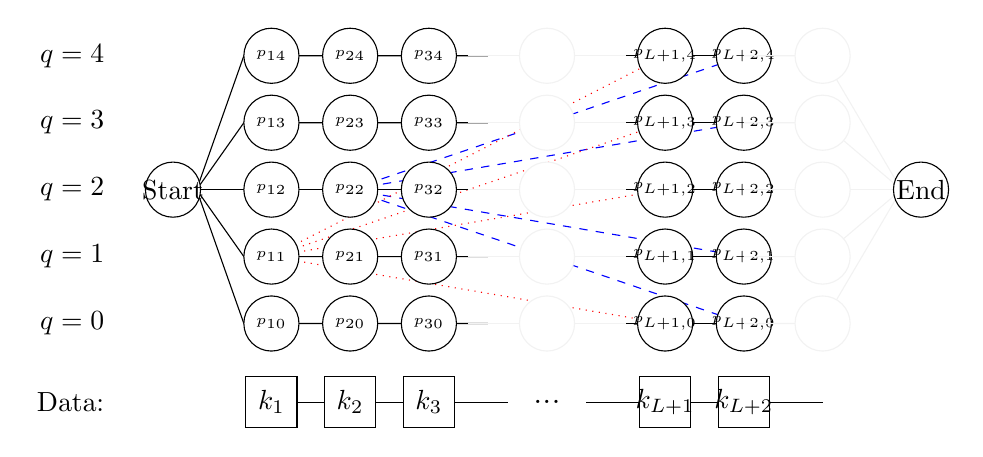
\begin{tikzpicture}
						
						\node[anchor=east] at (-2,0) {Data:};
						\draw (0,0)--++(3,0);
						\node at (3.5,0) {\large ...};
						\draw (4,0)--++(3,0);
						\def\w{0.65}
						\foreach \i in {1,...,3}
						{
							% \draw[fill=white] (\i-1,0) circle (0.35);
							\draw[fill=white] ({\i-1-\w/2},{\w/2})--({\i-1+\w/2},{\w/2})--({\i-1+\w/2},{-\w/2})--({\i-1-\w/2},{-\w/2})--cycle;
							\node at (\i-1,0) {$k_\i$};
						}
						
						
						\foreach \i in {1,...,2}
						{
							\draw[fill=white] ({\i+4-\w/2},{\w/2})--({\i+4+\w/2},{\w/2})--({\i+4+\w/2},{-\w/2})--({\i+4-\w/2},{-\w/2})--cycle;
							\node at ({4+\i},0) {$k_{L+\i}$};
						}
						
						\def\fac{0.85}
						
						\foreach \q in {0,...,4}
						{
							\def\y{\fac*\q+1}
							\if\q2
							\else
								\draw[dashed,blue] (1,{2*\fac+1})--(6,\y);
							\fi
							\if\q1
							\else
							\draw[dotted,red] (0,{1*\fac+1})--(5,\y);
							\fi
							% \if\q4
							% \else
							% \draw[dashdotted,green] (0,{4*\fac+1})--(5,\y);
							% \fi

						}
						\foreach \q in {0,...,4}
						{
							\def\y{\fac*\q+1}
							\draw (-0.95,{2*\fac+1})--(-0.35,\y)--(2.75,\y);
							\draw (4.25,\y)--(6,\y);
							\node[anchor=east] at (-2,\y) {$q=\q$};
							\foreach \i in {1,...,4}
							{
								\if\i4
									\def\c{gray!10!white}
									\draw[\c] (\i-1.5,\y)--++(2,0);
									\draw[\c,fill=white] (\i-0.5,\y) circle (0.35);
								\else
									\draw[fill=white] (\i-1,\y) circle (0.35);
									% \draw[fill=white] ({\i-1-\w/2},{\w/2})--({\i-1+\w/2},{\w/2})--({\i-1+\w/2},{-\w/2})--({\i-1-\w/2},{-\w/2})--cycle;
									\node at (\i-1,\y) {\tiny $p_{\i\q}$};
								\fi
								
							}
							\foreach \i in {1,...,3}
							{
								\if\i3
									\def\c{gray!10!white}
									\draw[\c] (\i+3,\y)--++(1,0)--(8,{2*\fac+1});
									\draw[\c,fill=white] (\i+4,\y) circle (0.35);
								\else
									\draw[fill=white] (\i+4,\y) circle (0.35);
									\node at (\i+4,\y) {\tiny $p_{L+\i,\q}$};
								\fi
								% \draw[fill=white] ({\i+4-\w/2},{\w/2})--({\i+4+\w/2},{\w/2})--({\i+4+\w/2},{-\w/2})--({\i+4-\w/2},{-\w/2})--cycle;
								% \node at ({4+\i},0) {$k_{L+\i}$};
							}
							
						}
						\draw[fill=white] (-1.25,{2*\fac+1}) circle (0.35);
						\node at (-1.25,{2*\fac+1}) {Start};
						\draw[fill=white] (8.25,{2*\fac+1}) circle (0.35);
						\node at (8.25,{2*\fac+1}) {End};


						
					\end{tikzpicture}
					}
					\caption{An example of a harmonic network -- only two sets of `jump edges' are shown (in red and blue) for clarity. In the full network, every node $p_{iq}$ is connected to $p_{i+1,q}$ and $p_{i+L,k\neq q}$. The graph is directional - vertices can only be traversed from left to right.}\label{F:Network}
				\end{center}
			
			\end{figure}

				After determining the value of the free parameters (discussed in Appendix \ref{A:Parameters}), Equations \eqref{E:NormBin} and \eqref{E:Prior} provide everything we need to compute the score \eref{E:Score} for a proposed set of $\{q\}$. The task of detecting the most likely (subject to our priors) set of copy-numbers is therefore equivalent to identifying the set of $\{q\}$ which maximise \eref{E:Score}. This is an integer optimisation problem, with the limiting factor that the dimensionality of the solution is equal to the chromosome size.
				% The Harmonic fitting method shows a vast improvement over the previous iteration - however it still suffers from a number of drawbacks, mostly associated with the somewhat dubious means by which the Bayesian tests were `bootstrapped' from each other (technically each successive probability should be fully conditioned on the previous set, rather than just stuffing that all into a simplistic prior).

				% The Harmonic Network method is an attempt to a) make the assignment robust and mathematically sound and b) devise a method which is conceptually easier to understand and follow. 

				Provided that we are able to make the assumption that there is some finite $Q$ such that $0 \leq q < Q$ across the entire genome, it is most convenient to think in terms of a \textit{network}, such that an assignment of $\{q\}$ corresponds to a unique path through the network: the optimal path is the one with the highest score.

				The network is arranged in a series of layers (not dissimilar in appearance to the network diagrams of feedforward neural networks), each layer corresponding to a given base in the genome. The vertices (or `nodes') in the layer then correspond to different values of $q$ that might be assigned to that base. In short, a path which passes a node $n_{iq}$ corresponds to the $i^\text{th}$ base being assigned a harmonic of $q$.

				The edges between vertices are directional, and obey the following rules, which are displayed graphically in Figure \ref{F:Network}:
				\begin{enumerate}
					\item The start node is connected to all nodes in the first layer, $n_{0,0\leq q < Q}$ 
					\item The node $n_{i,q}$ is connected to nodes $n_{j>i}$ through \textit{step edges} and \textit{jump edges}
					\begin{itemize}
						\item Step Edges connect $n_{i,q} \to n_{i+1,q}$, i.e. the same harmonic in the next layer. Step edges have a cost equal to
						\begin{equation}
							\text{Cost}(n_{iq} \to n_{i+1,q}) = p_{\vec{\theta}}(k_{i+1} | q) + \begin{cases} 0 & q = d_c \\  \mathfrak{p}_\text{ploidy} & \text{else} \end{cases}
						\end{equation}
						That is, they incur a cost equal to the posterior probability that $k_{i+1}$ arises from the same $q$ as $k_i$, the $\mathfrak{p}_\text{ploidy}$ is the prior probability that the $q$ is equal to the normal ploidy.
						\item Jump Edges connect $n_{i,q} \to n_{i+L,j\neq q}$, i.e. a different harmonic in a layer $L$ further along. This enforces the prior restriction that changes in $q$ must be above a certain length ($L$) in order to be considered valid. Jump Edges incur a cost equal to the posterior probabilty of assigning \textit{all} $k_{j}$ for $i < j \leq i + L$ to the new harmonic, and so the statistics must favour all of these $k$-values being assigned the same $q$ in order to consider a change in $q$ likely.
						\begin{equation}
							\text{Cost}(n_{iq} \to n_{i+L,j\neq q}) =\sum_{a = i+1}^{i+L} \left( p_{\vec{\theta}}(k_i | j) \right) +  \mathfrak{p}_\text{jump} + L \times  \begin{cases} 0 & j = d_c \\  \mathfrak{p}_\text{ploidy} & \text{else} \end{cases}
						\end{equation}
						We emphasise again that a path $n_{i,q} \to n_{i+L,j\neq q}$ means that $q_{i+1},....,q_{i+L}$ are all assigned the harmonic $j$, and that this is the only means by which a jump $q\to (j\neq q)$ is possible.
					\end{itemize}
					\item The nodes $n_{G-1,q}$ are connected to the End node
				\end{enumerate}
				
				Here we have used the shorthand $p_{\vec{\theta}}(k|q) = p(k| q^\prime\nu, \eta,\sigma,\gamma)$, our underlying distribution function given in \eref{E:NormBin}. From these rules it is a simple matter of using a basic shortest-path algorithm\footnote{{We are actually looking for the longest path, but minimising $|\mathcal{L}|$ is equal to maximising $\mathcal{L}$, so the distinction is trivial}}, using the associated cost of each node as the distance: step through each layer and compute the shortest path to each node in that layer, and then iterate until the end node is reached -- the longest path through this network corresponds to a unique $\{q\}$, which is then necessarily the one which maximses $\mathcal{L}$. An example of such a minimal path is shown in Fig. \ref{F:Path}.

				
				
				The runtime of this algorithm scales as $\mathcal{O}(Q^2 G)$, where $Q$ is the maximum harmonic and $G$ is the number of bases being evaluated. However, if we naively construct this network in-memory it occupies a space $m Q G$, where $m$ is the memory footprint of an individual node. {A conservative estimate of the naive implementation gives the memory requirements (for a human genome) of $\approx$650GB, well beyond what most consumer devices are capable of. We note, however, that the network is only semi-local -- the network does not need any information more recent than the previous $L+1$ nodes, and so the network can be constructed on-the-fly. With $L=10^5$, this reduces the memory requirements to a mere $\approx 35$MB. }
				
				% Assuming that $Q = 20$ and each node must know its score, $q$-value and a pointer to the previous node, this gives a conservative estimate of 646GB of active memory to construct a network for the entire human genome -- well beyond what most consumer devices are capable of. 

				% However, we note that this network is `semi-local' -- by design, the edges never extend beyond a distance $L$ from the current base. By placing node node $n_{iq}$ at index $C_{i \% (L+1),q}$, we only need $LQ$ nodes in memory at once, rather than $GQ$, a drastic reduction in memory footprint: $L = 10^5$ reduces the memory footprint to only 34MB.

				

				% However, we note that during the search for the value of $\nu$ (during which time many paths are evaluated, searching for the one which minimises $\mathcal{L}$), we only need the final `length' of the path, not the path itself. For the bulk of function calls to the path-tracing algorithm, therefore, we do not need to record the path - only its length -- and hence the runtime difference between the conveyor-belt algorithm and the naive algorithm is negligible, with the memory-footprint nevertheless vastly reduced.

				\begin{figure}
					\begin{center}
						\resizebox{!}{7.3cm}{ 
						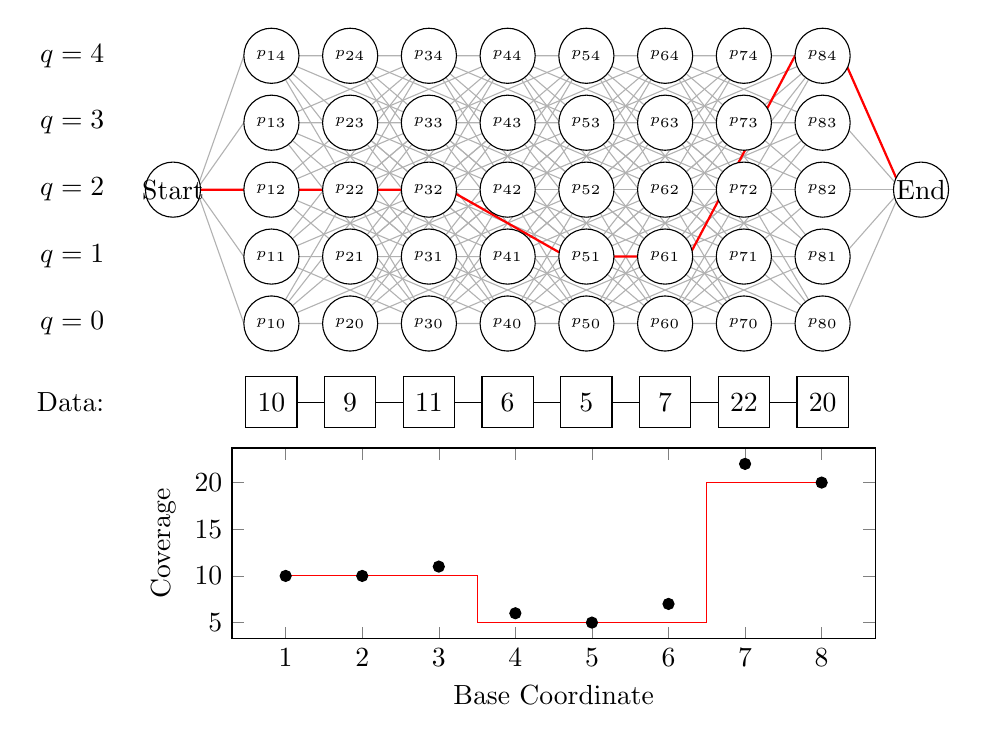
\begin{tikzpicture}
							
						%%network 
							\node[anchor=east] at (-2,0) {Data:};
							\draw (0,0)--++(7,0);
							\def\w{0.65}
							\foreach[count=\i] \j in {10,9,11,6,5,7,22,20}
							{
								% \draw[fill=white] (\i-1,0) circle (0.35);
								\draw[fill=white] ({\i-1-\w/2},{\w/2})--({\i-1+\w/2},{\w/2})--({\i-1+\w/2},{-\w/2})--({\i-1-\w/2},{-\w/2})--cycle;
								\node at (\i-1,0) {$\j$};
							}
							
							
							
							\def\fac{0.85}
							\foreach \q in {0,...,4}
							{
								\def\y{\fac*\q+1}
								\draw[black!30!white] (-0.95,{2*\fac+1})--(-0.35,\y)--(7.25,\y)--(8,{2*\fac+1});

								\foreach \i in {0,...,5}
								{
									\foreach \qq in {0,...,4}
									{
										\if\q\qq

										\else
											\draw[black!30!white] (\i,{\q*\fac+1})--(\i+2,{\qq*\fac+1});
										\fi
									}
								}
							}

							\draw[red,thick] (-0.95,{2*\fac+1})--(2.25,{2*\fac+1})--(3.75,{\fac+1})--(5,{\fac+1})--++(0.3,0)--(6.65,{4*\fac+1})--(7.25,{4*\fac+1})--(8,{2*\fac+1});
							
							\foreach \q in {0,...,4}
							{
								\def\y{\fac*\q+1}
								% \draw (4.25,\y)--(6,\y);
								\node[anchor=east] at (-2,\y) {$q=\q$};
								\foreach \i in {1,...,8}
								{
									
									\draw[fill=white] (\i-1,\y) circle (0.35);
									% \draw[fill=white] ({\i-1-\w/2},{\w/2})--({\i-1+\w/2},{\w/2})--({\i-1+\w/2},{-\w/2})--({\i-1-\w/2},{-\w/2})--cycle;
									\node at (\i-1,\y) {\tiny $p_{\i\q}$};
				
								}
								
								
							}
							\draw[fill=white] (-1.25,{2*\fac+1}) circle (0.35);
							\node at (-1.25,{2*\fac+1}) {Start};
							\draw[fill=white] (8.25,{2*\fac+1}) circle (0.35);
							\node at (8.25,{2*\fac+1}) {End};

						%%plot
							\begin{axis}[width=9.75cm,height=4cm,xlabel={Base Coordinate},ylabel={Coverage},at={(-0.5cm,-3cm)},scatter/classes={%
								a={mark=o,fill=black}}]
								\addplot[only marks,scatter src=explicit symbolic] table[row sep=crcr]{
									x y label \\
									1 10 a\\
									2 10 a\\
									3 11 a\\
									4 6 a\\
									5 5 a\\
									6 7 a\\
									7 22 a\\
									8 20 a\\
								};

								\addplot[red] table[row sep=crcr]{
									x y label \\
									1 10 a\\
									2 10 a\\
									3 10 a\\
									3.5 10 a\\
									3.5 5 a\\
									5 5 a\\
									6 5 a\\
									6.5 5 a\\
									6.5 20 a\\
									8 20 a\\
								};
								
								
							\end{axis}
						\end{tikzpicture}
						}
						\caption{(Top panel) A demonstration of an optimal path through a network with $L=2$ and $\nu=5$, given some example coverage data. (Bottom panel) a projection of this path back onto the coverage distribution. For aesthetic reasons we have placed the transitions at half-integers -- in practice non-integer values of base index are meaningless.}\label{F:Path}
					\end{center}
				\end{figure}



			\section{Results of the \codename{}}
			\begin{figure}
				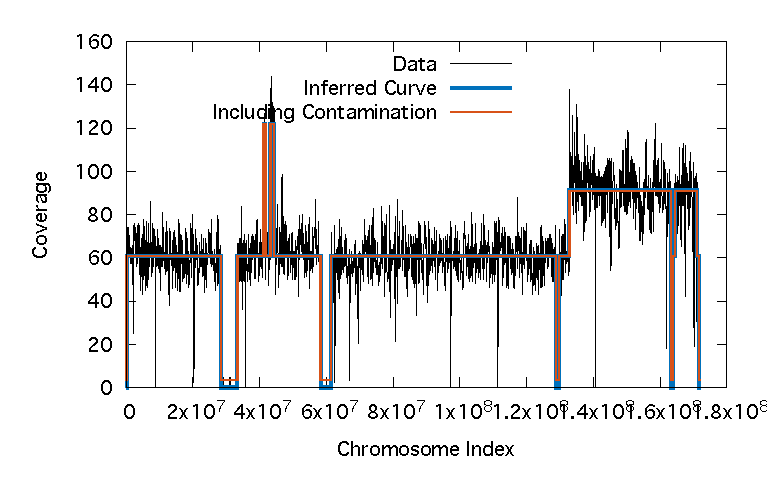
\includegraphics[height=6cm]{Figures/human_chr6.eps}
				\caption{The \codename{} predictions $q\nu$, (blue) for $L=2\times 10^5$bp overlaid onto a human oesophageal cancer sample (OES148, Chromosome 6, a known chromothripsis site). This chromosome has minimal contamination, and so the contamination-corrected curve $q^\prime \nu$ (red) shows only minor deviation. Recall that the blue curve is the most likely (large scale) copy number, and so is equal to an integer multiple, the red curve is the internal model used to derive the value of the blue curve. }\label{F:Human6}
			\end{figure}
			\begin{figure}
				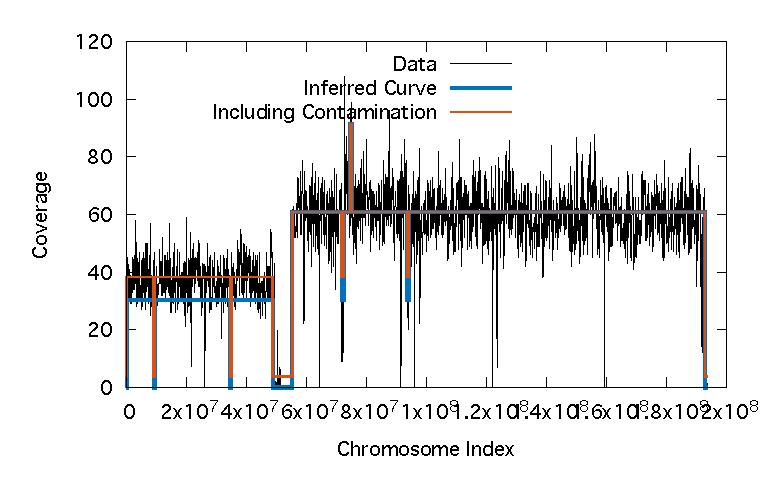
\includegraphics[height=6cm]{Figures/human_chr4.eps}
				\caption{The \codename{} predictions (blue) overlaid onto a human oesophageal cancer sample (OES148, Chromosome 4), demonstrating how the contamination-modelling shifts the position of the harmonic. Reported values (the blue curve)are always equal to $q \nu$, though the model internally uses $q^\prime \nu$, the contamination is assumed to be a laboratory artefact.}\label{F:Human4}
			\end{figure}


				\subsection{Human Oesophageal Cancer}
					In Figures \ref{F:Human6} and \ref{F:Human4} we show the results of the \codename{} algorithm applied to a human oesophageal chromothripsis cancer case, OES148, which was sequenced with {PacBio HiFi, a long-read sequencing technology}. Fig. \ref{F:Human6} is chromosome 6, known to be the main shattering site, and we see that the algorithm is indeed capable of identifying the large-scale changes present. {It is interesting to note which of the deletions the model considered valid - a human might consider the deletions at indices $10^7$, $\approx 10^8$ and $\approx 4 \times 10^8$ as important as those at $1.3\times10^8$ and $\approx 6\times 10^8$, however this is an artefact of the image compression - closer exmaination reveals this first set to be only a thousand bp in width, whilst the set that the algorithm identified are deletions in excess of $10^5$bp. \codename{} has therefore successfully performed as a data-reduction tool, preserving only those features which are most statisticaly meaningful.} 
					
					
					{Fig. \ref{F:Human4} shows chromosome 4 of the same sample.} This chromosome is not thought to be a major chromothripsis site, but we have included it in order to demonstrate the contamination-correction, since there is evidence that the $p$-end of one copy of chromosome 4 is deleted in a majority of cells in the sample, but not all of them -- we see that \codename{} has correctly identified that a partial aneuploidy (with a high degree of contamination) is the most likely explanation for the available data.
				
				% \begin{figure}
				% 	\includegraphics*[width=0.4\linewidth,keepaspectratio=true]{Figures/5.png}\includegraphics*[width=0.4\linewidth,keepaspectratio=true]{Figures/6.png}
				% \end{figure}

			{
			\subsection{Machine Learning \& Tasmanian Devils}

				We turn now to the case of Devil Facial Tumour Disease (DFTD), a transmissabel cancer affecting \textit{Sarcophilus harrisii}, the Tasmanian Devil\cite{Murchison2008,Murchison2012}, of which there are two distinct subtypes (DFT1, the original and most prevalent, and DFT2, a more recent, aggressive but rarer form)\cite{DFT22016}, and there is evidence that DFTD is caused by chromothripsis\cite{Deakin2012,Stammnitz2023}. 

				The goal of the \codename{} is not merely to serve as a copy-number analyser for its own sake, but as a preprocessing layer with the goal of converting the extremely large, extremely noisy coverage data into a meaningful encoding for use in Machine Learning. 	Due to the genetic homogeneity of both Tasmanian Devils as a whole, and of DFTD, this provides us with a useful proof-of-concept for \codename{} in coverage-based cancer inference.
				
				
				\codename{} is intended to serve as an initial transformation of the data (an input layer) for traditional Machine Learning methods. The Machine Learning models we present, therefore, are intentionally simple and out-of-the-box, in order to prove that the \codename{} has succeeded in preserving the large scale behaviour of the data over the course of its data reduction. 

				Using a dataset of 177 Tasmanian Devils\cite{Stammnitz2023} sequenced using standard Illumina Short Read sequencing, and annotated as being either 'normal' (i.e. non-cancerous), 'DFT1' or 'DFT2', we transformed the data using \codename{}, and encoded the data into a 20-dimensional feature vector, as described in Appendix \ref{A:Vector}.

				We then used a simple Feedforward Neural Network (5 layers, dimensions 20,30,10,8,3, ReLu activation throughout) as a classifier, including a 50\% dropout layer after the second layer to prevent overfitting. This model is a standard implementation -- the novelty of our method is in the input layer and the feature representation, not the ML model itself.

				In Fig. \ref{F:Classifier} we show the result of the accuracy of this classifier: it exceeded 95\% accuracy everywhere, indicating that the encoding is retaining the information necessary to detect cancer-causing SVs, and to identify which SVs are responsible for which cancer. We note that there were a number of troublesome misclassifications; investigating the dataset revealed a number of low-quality sequences from early in the data collection programme. Future work shall incorporate additional information into the \codename{} output and subsequent encoding to allow the identification of such artefacts, and hence allow the classifier to focus on the cancer signal. 

				Unsupervised methods yielded similarly positive results. In the right panel of Fig. \ref{F:Classifier}, we demonstrate the result of a UMAP clustering\cite{UMAP2018} on a $N=200$ encoding of our dataset. The result is a spectacular dissection of the feature space: aside from two misclassifications, UMAP correctly clustered all of the non-cancerous, DFT1 and DFT2 datasets into isolated clusters. 
			
				In addition, we notice that there is additional substructure present: the 'normal' datasets are bifurcated, investigation revealed this to be based solely on the sequencing depth of the sex chromosomes (the normal set contained both male and female Devils); however (since the transmissable cancer is spread primarily through male-male sexual competition), the cancer samples are entirely male. The subtypes within the DFT2 cluster, arises from substructure within DFT2, where two distinct clades have already been identified\cite{Stammnitz2023} - our clusterings match up with the assigned clades with other methods. That the DFT1 cluster is does not similarly split up into the 6 clades identified elsewhere is most likely a feature of our (somewhat naive) encoding, the loci which differentiate the clades would fall within the same spatial bin, and so do not permit the separation of the clades. We have begun work on a more nuanced encoding which would permit such spatial resolution within the encoding.


				The work in this section is preliminary, and serves only to demonstrate that the \codename{} algorithm has great potential as a data reduction and transformation tool for future Machine Learning work, which we intend to include novel encodings and architectures.
		

				\begin{figure}
					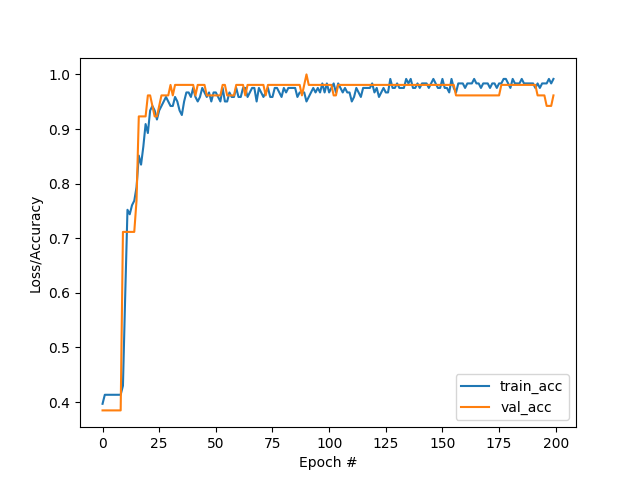
\includegraphics[width=0.55\linewidth]{Figures/Classifier.png}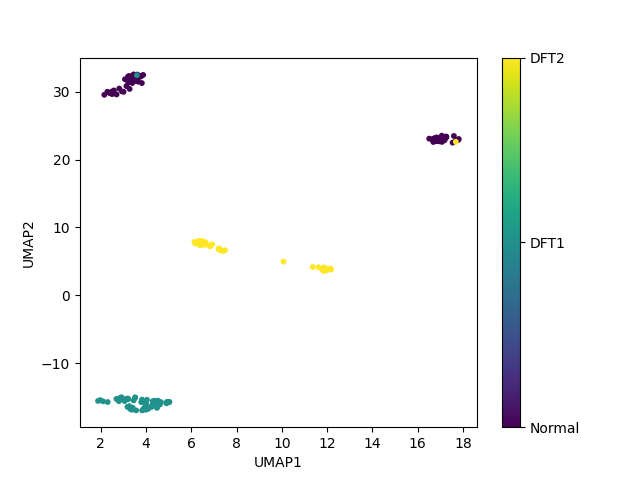
\includegraphics[width=0.55\linewidth]{Figures/UMAP.png}
					\caption{(\textit Left: )The accuracy of a 5-layer FNN with a 50\% dropout rate after the second layer. We see a convergence to extremely high prediction accuracy. (\textit{Right}:) a UMAP clustering of the Tasmanian Devil dataset}\label{F:Classifier}
				\end{figure}

			}
			\section{Conclusions \& Future Work}
					
					In this work we have demonstrated the \textit{\codename{}} algorithm, a powerful data-reduction method based on the principles of step-detection. \codename{} permits us to incorporate the effects of biological variability, contamination and minimum jump-sizes to retain only the most statistically important deviations from the expected ploidy, and works equally well on both long and short read technologies.  \codename{} is publicly available: \url{https://github.com/wtsi-hpag/GenCHORD}

					We have demonstrated that this method permits us to transform the high-dimensional and complex data associated with Tasmanian Devil Facial Tumour Disease into a low-dimensional representation from which a small 5-layer FNN model can learn, with unerring accuracy, to predict the presence and type of cancer. We also showed that the \codename{} preserved information by which an unsupervised method could cluster the cancers into familiar groupings, but also uncover new subtypes, the nature of which we are still investigating. 
					
					This proves a useful testbed of \codename{} as a tool for studying cancer, however, the exact properties which make Tasmanian Devils an attractive test case of this method (the genetic homogeneity of the population and near-clonality of the cancer) mean that application to the human case will be far from trivial. 

					Future work on this topic will focus on the encoding methodology and novel ML architecture: how this reduced data can be represented in the machine in such a way to make feature extraction meaningful, explainable and useful for scientific and diagnostic applications. 
					
			
				\bibliography{references.bib}
			\appendix
			{\small 
			\section{Mathematical Theory}\label{A:Theory}
				\subsection{Negative Binomial}
					The statistical model $\mathcal{P}$ for the coverage $k$, is derived from the common assumption that the genome is sampled via a Poisson distribution with mean $\lambda$, but where there are biological and experimental errors which change $\lambda$, such that the model is the convolution of a Poisson distribution, and some 'error distribution', which encodes the degree to which $\lambda$ varies. Whilst maximal-entropy arguments might imply a lognormal distribution as the optimal choice, for convenience (since the outcome is analytically computable), we use the Gamma distribution with mean $\mu > 0$ and variance $\sigma^2 > 0$, which gives the Negative Binomial Distribution as our model:
					\begin{align}
						\mathcal{P} & = \int_0^\infty \Gamma(\lambda| \mu,\sigma) \text{Poisson}(k|\lambda) \d \lambda \LLR k \sim\text{NB}\left(k; \mu, \mu + \sigma^2\right) 
					\end{align}

					We make a modification to this model, since it will often be necessary to truncate the probability distribution to some finite $K$ to avoid contamination with short but highly repetitive regions which fall outside the scope of our model. We therefore normalise the model up to this finite $K$:
					\begin{equation}
						p(k; \mu, \mu+\sigma^2) = \frac{\text{NB}\left(k; \mu, \mu + \sigma^2\right)}{\sum_{k^\prime = 0}^K \text{NB}\left(k^\prime; \mu, \mu + \sigma^2\right) } \label{E:NormBin}
					\end{equation}

				\subsection{Statistical Model}\label{A:Model}

					The task of idenitfying breakpoints is equivalent to assigning $\{q\}$-values to a given genome. We must therefore form statistical score $\mathcal{L}(\{q\})$, which is maximised at the most likely set $\{q\}$. We make the standard assumption that the coverage $k_i$ of the $i^\text{th}$ base is drawn independently and identically from an underlying distribution function (\textit{iid}), which is a function of the fundamental frequency, $\nu$, and the harmonic, $q_i$. Bases are statistically connected through the \textit{prior} function, which encodes many of the points outlined in the previous section. As a result of the \textit{iid} assumption, the global score can be found to be:
			
					\begin{align}
						\mathcal{L}(\{q\} | \{k\}, \nu,\sigma,\vec{\theta}) & = \sum_i \mathfrak{p}\left(k_i | q_i, \nu,\sigma \right) + \text{Prior}(\{q\},\vec{\theta}) \label{E:Score}
					\end{align}
					Here $\vec{\theta}$ are the hyperparameters of the model. This is an indirect statement of standard Bayesian Maximum Posterior methodology - the quantity $\mathfrak{p}$ is the log-probability of observing the data $k_i$ given the harmonic $q_i$ and parameter $\nu$; as already discussed, this will take the form of a Negative Binomial distribution. Finally, we must formulate a suitable prior, which enforces the remainder of our assumptions, namely:
					\begin{enumerate}
						\item Consecutive values of $q_i$ should be similar
						\item Changes in $q_i$ can only happen over a large distance
						\item Most of the chromosome $c$ should be at $q_i = d_c$ (equal to the ploidy)
					\end{enumerate}
					Therefore, we propose:
					\begin{spalign}
						\text{Prior}(\{q\})   = & \sum_i \Bigg[  \mathfrak{p}_\text{ploidy} u(q_i,d_c)  + u(q_i,q_{i-1})\left( \mathfrak{p}_\text{jump} +  \mathfrak{p}_\infty \sum_{j = i-L}^{i-1} u(q_j,q_{i-1})  \right)\Bigg]
						\\
						u(a,b)  = & (1-\delta_{ab}) = \begin{cases}
							0 & {a = b}
							\\
							1 & \text{else}
						\end{cases}\label{E:Prior}
					\end{spalign}
					The terms in the prior therefore act (in order), to penalise every base which is not at the expected diploid level by an amount $\mathfrak{p}_\text{diploid}$, penalise every jump between dissimilar $q$s by an amount $\mathfrak{p}_\text{jump}$ and to penalise jumps which occur within a distance $L$ of another jump by an amount $\mathfrak{p}_\infty$, which is a number $\approx -\infty$, but which has the property $0 \times \mathfrak{p}_\infty = 0$ -- rather than a penalty, this therefore acts as a \textit{forbiddance}, discarding models with such jumps.

		\section{Parameter Inference}\label{A:Parameters}


			The model presented above has a number of free parameters - notably $\nu$ (the fundamental sampling frequency of the chromosome), $\sigma$ (the standard deviation of the sampling-noise function), $\gamma$ (the degree of alignment noise), $\eta$ (the contamination amount), as well as the functional form of $p_\text{error}$.

			We need to determine these values before we may reliably assign the values of $\{q\}$. To do this efficiently, we shall assign these values based on the global coverage distribution - the counts of all observed coverage values binned into a histogram. To this distribution, we then fit a Negative Binomial Mixture Model using the contamination-biased probability:
			\begin{equation}
				p_\text{global}(k|\vec{\theta}) = \gamma p_\text{error}(k) + (1-\gamma)\sum_{q=0}^Q w_q NB\left(k_i; q^\prime(q,\eta) \nu, \sigma\right)
			\end{equation}
			Where $w_q$ are the population weightings; equal to the fraction of bases which will be assigned to $q$ when the full assignment is performed. \codename{} uses a standard Maximum Posterior Method to infer the maximal value of these parameters given a set of data.

		\section{Feature Vector}\label{A:Vector}

			After the data has been reduced by \codename{}, we encode it into a feature vector $\vec{v}$ of length $N$. Each element of the vector corresponds to a portion of the genome of length $G/N$ where $G$ is the total length of the genome. Each segment is assigned a score based on the presence, $q$-value and length of domains that GeneCHORD had assigned, where a domain is a continuous region of length $\ell$ which has been assigned the same value of $q$. The score associated with a domain $D(\ell,q)$ on chromosome $c$ (which has ploidy $d_c$) is:
			\begin{equation}
				S(\ell,q,d_c) = \exp\left(|q - d_c| + \frac{\ell N}{G}\right)
			\end{equation}
			The score assigned to each element of the feature vector $\vec{v}$ is then the sum of scores for all domains in the associated portion of the genome.
			

		}
		% \section{Parameter Optimisation}


		% 	Although it would be possible to infer the values of $\nu, \sigma,\gamma,\mu_e,\sigma_e$ by optimising them against \eref{E:Score}, this is computationally quite intensive - since it involves multiple passes through the network to explore this multidimensional parameter space. It is therefore much easier to fit these global parameters to the \textit{global distribution} of coverages, before then using them to infer the \textit{local} values of $q_i$.

		% 	If we truncate the data to only look at $k$ up to some maximum value $K$, the global distribution function is equal to:
		% 	\begin{spalign}
		% 		p_\text{global}(k|\vec{\theta}) & = \sum_q w_q p_{\vec{\theta}}(k|q,K)
		% 		\\
		% 		& =  \sum_q w_q \frac{p_{\vec{\theta}}(k|q)}{\sum_{k^\prime = 0}^K p_{\vec{\theta}}(k|q)}
		% 		% & = \gamma {NB}\left(k; \frac{\mu_e^2}{\sigma_e^2}, \frac{\mu_e}{\mu_e + \sigma_e^2} \right)
		% 		% \\
		% 		% & ~~~~~ + (1-\gamma)\sum_q w_q {NB}\left(k; \frac{(q\nu)^2}{\sigma^2}, \frac{q\nu}{q\nu + \sigma^2} \right) 
		% 	\end{spalign}
		% 	Where $w_q$ are the weights associated with each of the subpopulations; rather than assignined each base to a given $q$ were are fitting them as an aggregate population.	The Bayesian score associated with data binned such that $N_k$ is the number of bases assigned the coverage $k$ is then:
		% 	\begin{align}
		% 		\mathcal{L}_\text{global} & = \mathcal{P}(\vec{\theta}) + \sum_k N_k \ln\left(p_\text{global}(k|\vec{\theta})\right)
		% 		\\
		% 		& =\mathcal{P}(\vec{\theta}) + \sum_k N_k \ln\left(\sum_q w_q p_{\vec{\theta}}(k|q)\right) - N \ln\left(\sum_k \sum_q w_q p_{\vec{\theta}}(k|q)\right) 
		% 	\end{align}
		% 	Where $N = \sum_k N_k$ is the total number of observations. The parameters are then optimised using the gradients:
		% 	\begin{spalign}
		% 		\pdiv{\mathcal{L}}{\theta_i} = \pdiv{\mathcal{P}}{\theta_i} + \sum_k \sum_q\left(\frac{N_K}{\sum_q w_q p(k|q)} - \frac{N}{\sum_{k,q} w_q p(k|q)}\right) w_q\pdiv{p(k|q)}{\theta_i}
		% 	\end{spalign}
		% 	Using the shorthand
		% 	\begin{equation}
		% 		R_k = \left(\frac{N_K}{\sum_q w_q p(k|q)} - \frac{N}{\sum_{k,q} w_q p(k|q)}\right)
		% 	\end{equation}
		% 	This can be simplified to
		% 	\begin{spalign}
		% 		\pdiv{\mathcal{L}}{\theta_i} & = \pdiv{\mathcal{P}}{\theta_i} + \sum_k \sum_q R_k  w_q\pdiv{p(k|q)}{\theta_i}
		% 		\\
		% 		\pdiv{\mathcal{L}}{w_q} & = \pdiv{\mathcal{P}}{w_q} + \sum_k R_k  p(k|q)
		% 	\end{spalign}
		% 	However, since we must maintain that $\sum_q w_q = 1$ and $0 < w_q < 1$, it is convenient to reparameterise this as $w_i = e^{z_i}/\sum_j e^{z_j}$, such that
		% 	\begin{spalign}
		% 		\pdiv{L}{z_i} & = w_i \left(\pdiv{\mathcal{P}}{w_i} + \sum_k R_k p(k|q) - \sum_j w_j \left[\pdiv{\mathcal{P}}{w_j} + \sum_k R_k p(k|j)\right]\right)
		% 	\end{spalign}
		% 	% Where (using the notation that $B_{kq} = {NB}\left(k; \frac{(q\nu)^2}{\sigma^2}, \frac{q\nu}{q\nu + \sigma^2}\right) $, $E_k = {NB}\left(k; \frac{\mu_e^2}{\sigma_e^2}\right)$, $r_e = \frac{\mu_e^2}{\sigma_e^2}$, $p_e = \frac{\mu_e}{\mu_e + \sigma_e^2}$, $r_q = \frac{\nu^2 q^2}{\sigma^2}$ and $p_q = \frac{q\nu}{q\nu + \sigma^2}$)
		% 	% \begin{spalign}
		% 	% 	\pdiv{p_k}{\gamma} & = {E}_k - \sum_q w_q {B}_{kq}
		% 	% 	\\
		% 	% 	\pdiv{p_k}{z_j} & = (1-\gamma) w_j \left[ B_{kj} - \sum_q w_q B_{kq} \right]
		% 	% 	\\
		% 	% 	\pdiv{p_k}{\mu_e} & = \gamma E_k \Big[ \frac{2\mu_e}{\sigma_e^2} \left(\psi\left(k + r_e\right) + \ln\left(p_e\right) - \psi\left(r_e\right) \right)
		% 	% 	\\
		% 	% 	&~~-\frac{\sigma_e^2}{(\mu_e + \sigma_e^2)^2} \frac{p_e (k+r_e) - r_e}{p_e^2} \Big]
		% 	% 	\\
		% 	% 	\pdiv{p_e}{\sigma_e} & = 2\gamma E_k \Big[ \frac{\sigma_e}{(\mu_e + \sigma_e^2)^2} \frac{p_e (k+r_e) - r_e}{p_e^2} 
		% 	% 	\\
		% 	% 	& ~~- 2\frac{\mu_e^2}{\sigma_e^3} \left(\psi\left(k + r_e\right) + \ln\left(p_e\right) - \psi\left(r_e\right) \right)\Big]
		% 	% \end{spalign}
		% 	% \begin{spalign}
		% 	% 	\pdiv{p_e}{\nu} & = (1-\gamma) \sum_q w_q B_{kq}  \Big[ \frac{2\nu q^2}{\sigma^2} \left(\psi\left(k + r_q\right) + \ln\left(p_q\right) - \psi\left(r_q\right) \right)
		% 	% 	\\
		% 	% 	&~~-\frac{\sigma^2}{(q\nu + \sigma^2)^2} \frac{p_q (k+r_q) - r_q}{p_q^2} \Big]
		% 	% 	\\
		% 	% 	\pdiv{p_e}{\sigma} & = 2(1-\gamma) \sum_q w_q B_{kq} \Big[ \frac{\sigma}{(q\nu + \sigma^2)^2} \frac{p_q (k+r_q) - r_q}{p_q^2} 
		% 	% 	\\
		% 	% 	& ~~- 2\frac{q^2\nu^2}{\sigma^3} \left(\psi\left(k + r_q\right) + \ln\left(p_q\right) - \psi\left(r_q\right) \right)\Big]
		% 	% \end{spalign}
			

\end{document}
